\infannex{introProg}{Introduction for Programmers}

\tikzset{  
block/.style    = {draw, thick, rectangle, minimum height = 3em, minimum width = 3em},}

\pnum
\rSec1[introProg.sw]{Software}

In software, the core model is the time-multiplexed execution
of software threads by one or more central processing units (CPUs).
Extensive use of address arithmetic (pointers
and indexing) improves code density, both at the source level and at
runtime.

The programmer
must decorate the code with library calls to dynamically enforce
mutual exclusion (mutex) regions, preventing the interleaved execution of
multiple threads accessing a single storage element.
In languages like Java, the programmer is able to decorate the
storage element declarations to automate calling of these mutex operations.

In all cases, since the compiler cannot statically determine which specific
storage elements are subject to contentious access, the programmer is responsible
for correct manual decoration of the source code.

%%%%%%%%%%%%%%%%%%%%%%%%%%%%%
    \begin{tikzpicture}
        [title/.style={font=\fontsize{18}{18}\color{black!45}},
        server/.style={rectangle, draw, fill=blue!23, rounded corners, minimum height=9em},
        client/.style={rectangle, draw, fill=green!23, rounded corners, minimum height=2em},
        dot/.style={circle, fill=black, minimum size=2pt, inner sep=0pt, outer sep=2pt},
        link/.style={latex-latex}]
        % Place nodes
        \node [server, outer sep=8pt, align=center] (s1) at (5,8.3) {S1};
        \node [server, outer sep=8pt, align=center] (s2) at (7.65,8.3) {S2};
        \node [server, outer sep=8pt] (s3) at (10.3,8.3) {S3};
        \node [draw=black!50, fit={(s1) (s2) (s3)}] (back) {};
        \node [client] (c1) at (0,9.5) {C1};
        \node [client] (c2) at ($(c1) + (270:1.15)$) {C2};
        \node [client] (c3) at ($(c2) + (270:1.15)$) {C3};
        \node [dot] (c4) at ($(c3) + (270:1)$) {};
        \node [dot] (c5) at ($(c4) + (270:0.5)$) {};
        \node [dot] (c6) at ($(c5) + (270:0.5)$) {};
        \node [draw=red!50, fit={($(c1.north)+(0, 8pt)$) (c2) (c3) (c4) (c5) ($(c6.south)+(0, -7pt)$)}, inner sep=5.75pt] (front) {};
        \draw (c1) -- (c1-|back.west)
            (c2) -- (c2-|back.west)
            (c3) -- (c3-|back.west);
        % Place edges
    \end{tikzpicture}


%%%%%%%%%%%%%%%%%%%%%%%%%%%%%
test2

\begin{tikzpicture}[
	decoration={ markings, mark=at position 1cm with {\arrow[black]{stealth}}, },
	path/.style={ ->, >=stealth, postaction=decorate },
	every node/.style={font=\sffamily}
]
\node [ draw, yshift=2cm, minimum width=4cm, ] (control) {Control System};
\node [ draw, minimum width=5cm, minimum height=1cm, ] (process) {Process/Equipment};
\node [ draw, yshift=-2cm, minimum width=4cm, ] (safety) {Safety System}; 

\draw[path] (control.east) -- ++(1,0) |- ([yshift=-0.25cm] process.north east);
\draw[path] ([yshift=-0.25cm] process.north west) -- ++(-1,0) |- (control.west);
\draw[path] ([yshift=0.25cm] process.south west) -- ++(-1,0) |- (safety.west);
\draw[path] (safety.east) -- ++(1,0) |- ([yshift=0.25cm] process.south east);

\end{tikzpicture}
%%%%%%%%%%%%%%%%%%%%%%%%%%%%%

\tikzstyle{b} = [rectangle, draw, fill=blue!20, node distance=1cm, text width=6em, text centered, rounded corners, minimum height=2em, thick]
\tikzstyle{c} = [rectangle, draw, inner sep=0.1cm, dashed]
\tikzstyle{l} = [draw, -latex',thick]

\begin{tikzpicture}[auto]
    \node [b] (planning) {Planning};
    \node [b, below=of planning] (resources) {Resources};
    \node [b, below=of resources] (sensors) {Sensors};
    \coordinate (RSmid) at ($(resources.south west)!0.5!(sensors.north west)$);
    \node [b, left=of RSmid, node distance=4cm] (information) {Information system};
    \node [b, below=of sensors] (processing) {Processing};

    \node [c,fit=(resources) (sensors)] (container) {};

    \path [l] (planning) -- (resources);
    \path [l] (resources) -- (sensors);
    \path [l] (sensors) -- (processing);

    \path [l] (information) |- (planning);
    \path [l] (information) |- (processing);

    \node at (container.north west) [above right] {Desc};

    \draw [l] (processing.east) -- ++(2,0) node(lowerright){} |- (planning.east);
    \draw [l] (lowerright |- container.east) -- (container.east -| resources.south east);
\end{tikzpicture}

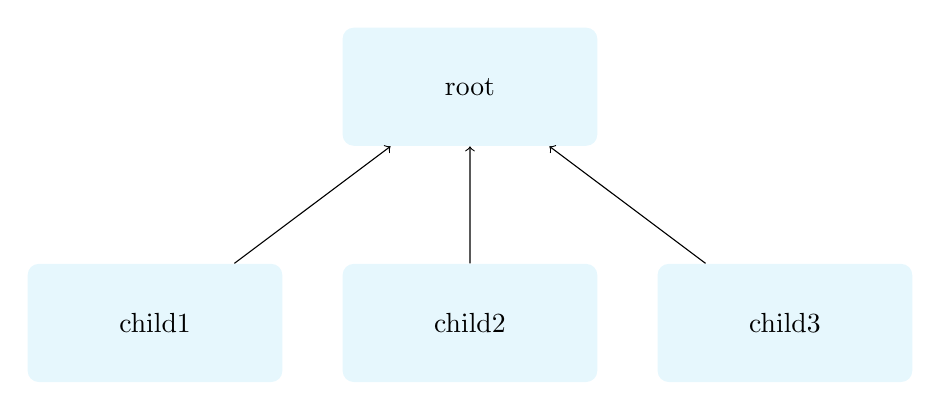
\begin{tikzpicture}
    \tikzset{block/.style={rectangle, fill=cyan!10, text width=3cm, text centered, rounded corners, minimum height=1.5cm}};
    \node[block] {root} [level distance=3cm, sibling distance=4cm, edge from parent/.style={<-,draw}]
        child{ node[block] {child1} }
        child{ node[block] {child2} }
        child{ node[block] {child3} };
\end{tikzpicture}

\begin{tikzpicture}[auto, thick, >=triangle 45,fill=blue!20]
\node at (0,0)[block,draw,fill=blue!20] (clogic) {Scheduler};
\node[block,below of=clogic,node distance=2cm,fill=blue!20] (memory) {CPU};
\draw[<-] ([yshift=2ex]clogic.west) to node[midway,above] {$Input$} ++(-3,0);
\draw[->] ([yshift=2ex]clogic.east) to node[midway,above] {$Output$} ++(3,0);
\draw[->] ([yshift=-2ex]clogic.east) -| node[midway,right] {$Next State$} ([xshift=60]memory.east)
                                    |- (memory.east);
\draw[->] (memory.west) -| ([xshift=-60]memory.west)
                       |- node[midway,left] {$Current State$} ([yshift=-2ex]clogic.west);
\draw[<-] (memory.south) to ++(0,-1) node[below] {$Clock$};
\end{tikzpicture}

\rSec1[introProg.hw]{Hardware}

In hardware, the core model is clock-based updates to state elements from
a combinational logic net.

Combinational logic = current output is a boolean combination of current inputs

Sequential logic = combinational logic + memory elements
(also called finite-state machine)

Synchronous logic = sequential logic + clock

\begin{tikzpicture}[auto, thick, >=triangle 45,fill=blue!20]
\node at (0,0)[block,draw,fill=blue!20] (clogic) {Combinational Logic};
\node[block,below of=clogic,node distance=2cm,fill=blue!20] (memory) {Memory};
\draw[<-] ([yshift=2ex]clogic.west) to node[midway,above] {$Input$} ++(-3,0);
\draw[->] ([yshift=2ex]clogic.east) to node[midway,above] {$Output$} ++(3,0);
\draw[->] ([yshift=-2ex]clogic.east) -| node[midway,right] {$Next State$} ([xshift=60]memory.east)
                                    |- (memory.east);
\draw[->] (memory.west) -| ([xshift=-60]memory.west)
                       |- node[midway,left] {$Current State$} ([yshift=-2ex]clogic.west);
\draw[<-] (memory.south) to ++(0,-1) node[below] {$Clock$};
\end{tikzpicture}

From Hoe\cite{Hoe:Thesis}, the Term Rewriting System representation of this is:

$\textbf{s'}$ = if $\pi(\textbf{s})$ then $\delta(\textbf{s})$ else $\textbf{s}$

Since all hardware elements are independent, all valid source lines in the
program text are executed on every cycle.
Access to state elements supports neither pointers nor indexing, allowing the
compiler to statically determine parallel access transaction conflict sets,
allowing the flagging of all combinations where correct operation cannot
be guaranteed.
